\section{Introduction}

\begin{figure}[t]
  \begin{center}
  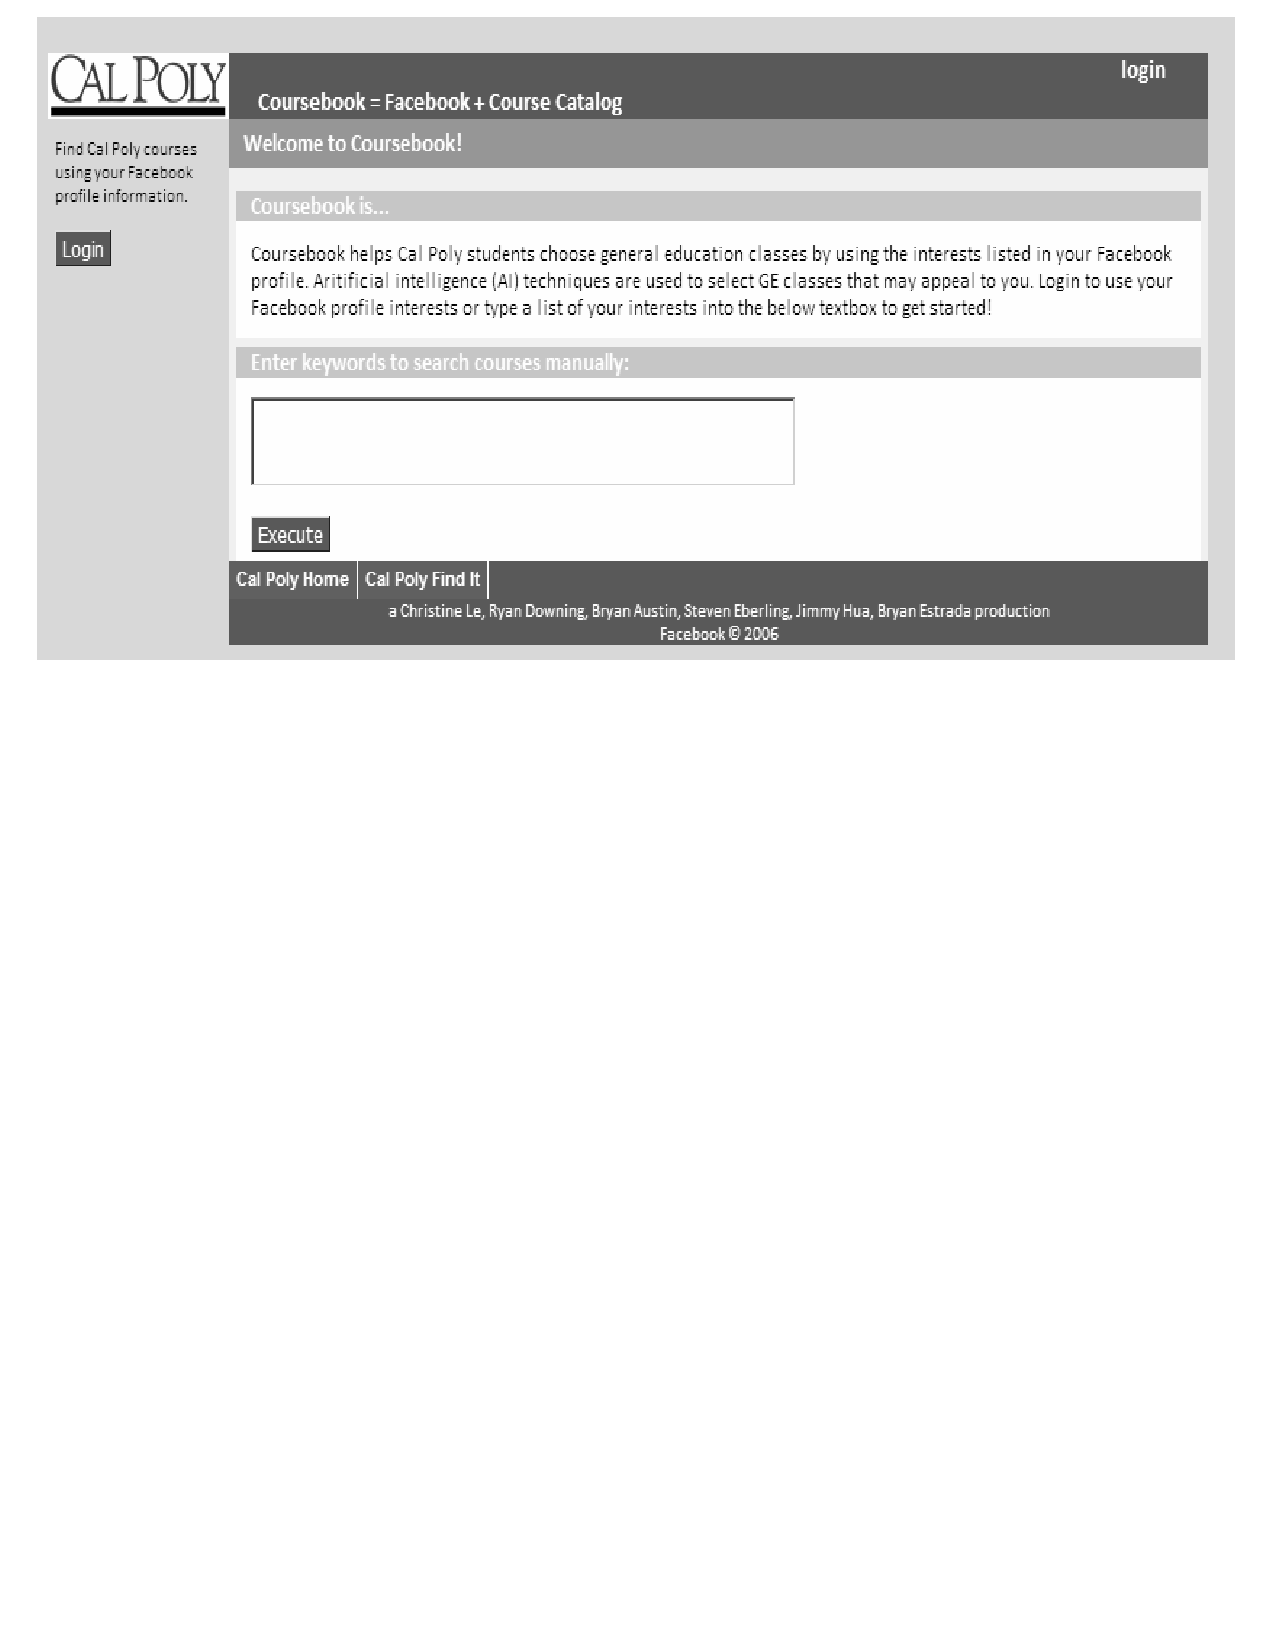
\includegraphics[scale=0.75]{images/screenshot}
  \caption{Coursebook Screenshot}
  \label{fig:screenshot}
  \end{center}
\end{figure}

Coursebook is a Facebook enabled website that provides general education course
recommendations to its users. Facebook is an online social network that allows
people to connect with others through schools, companies, regions and groups.
Coursebook utilizes a relational database of course offerings for California 
Polytechnic State University students to provide this service. Coursebook is a multi-
threaded, highly-concurrent web service built on the J2EE platform. By drawing 
from Facebook's user interests and profile information, Coursebook searches for 
general education classes would be most appealing to each user. The main task of 
the system is to provide its users with relevant general education courses based on 
their personal interests. Figure \ref{fig:screenshot} is a screenshot of the
Coursebook website.

The intended domain is academic, targeting Cal Poly students seeking to enroll 
in general education courses. This service gives students an alternative way of 
finding general education courses that may interest them, rather than manually 
searching through the long list of available classes in the Cal Poly course catalog. 
Coursebook also provides the option of manually entering a student's interests 
through a web form to search for relevant courses, allowing more flexibility and 
functionality to its users. Coursebook aims to provide a service that is:

\singlespacing
\begin{itemize}
  \item easily accessible,
  \item highly responsive,
  \item fault tolerant,
  \item platform agnostic, and
  \item maintainable for the future.
\end{itemize}
\doublespacing

Coursebook was designed using several different design patterns. A design 
pattern represents a solution to a common problem. The knowledge for that 
particular problem is encapsulated into a design pattern, allowing for those who 
must address the problem in the future to build upon the existing knowledge to 
better solve the problem. There exists many fundamental design patterns that are 
commonly used across all software design projects. Coursebook utilizes several of 
these patterns, including the Singleton, Iterator, and Command. Design patterns 
that address specific problems in certain domains have also been developed. 
Coursebook makes use of a few of the design patters meant for distributed and 
concurrent systems. These patterns include the Active Object pattern and the 
Leader/Follower pattern. Coursebook is currently live and fully functional and is 
based upon these design patterns. It can be reached at 
\verb!http://ghoul.csc.calpoly.edu!. Future work on Coursebook includes
modifying the design to include the Pipeline and Recoverable Distributor
patterns, to add client-side concurrency, improve user perceived response time,
improve fault tolerance, and improve reliability.

\section{Requirements}

\begin{figure}[t]
  \begin{center}
  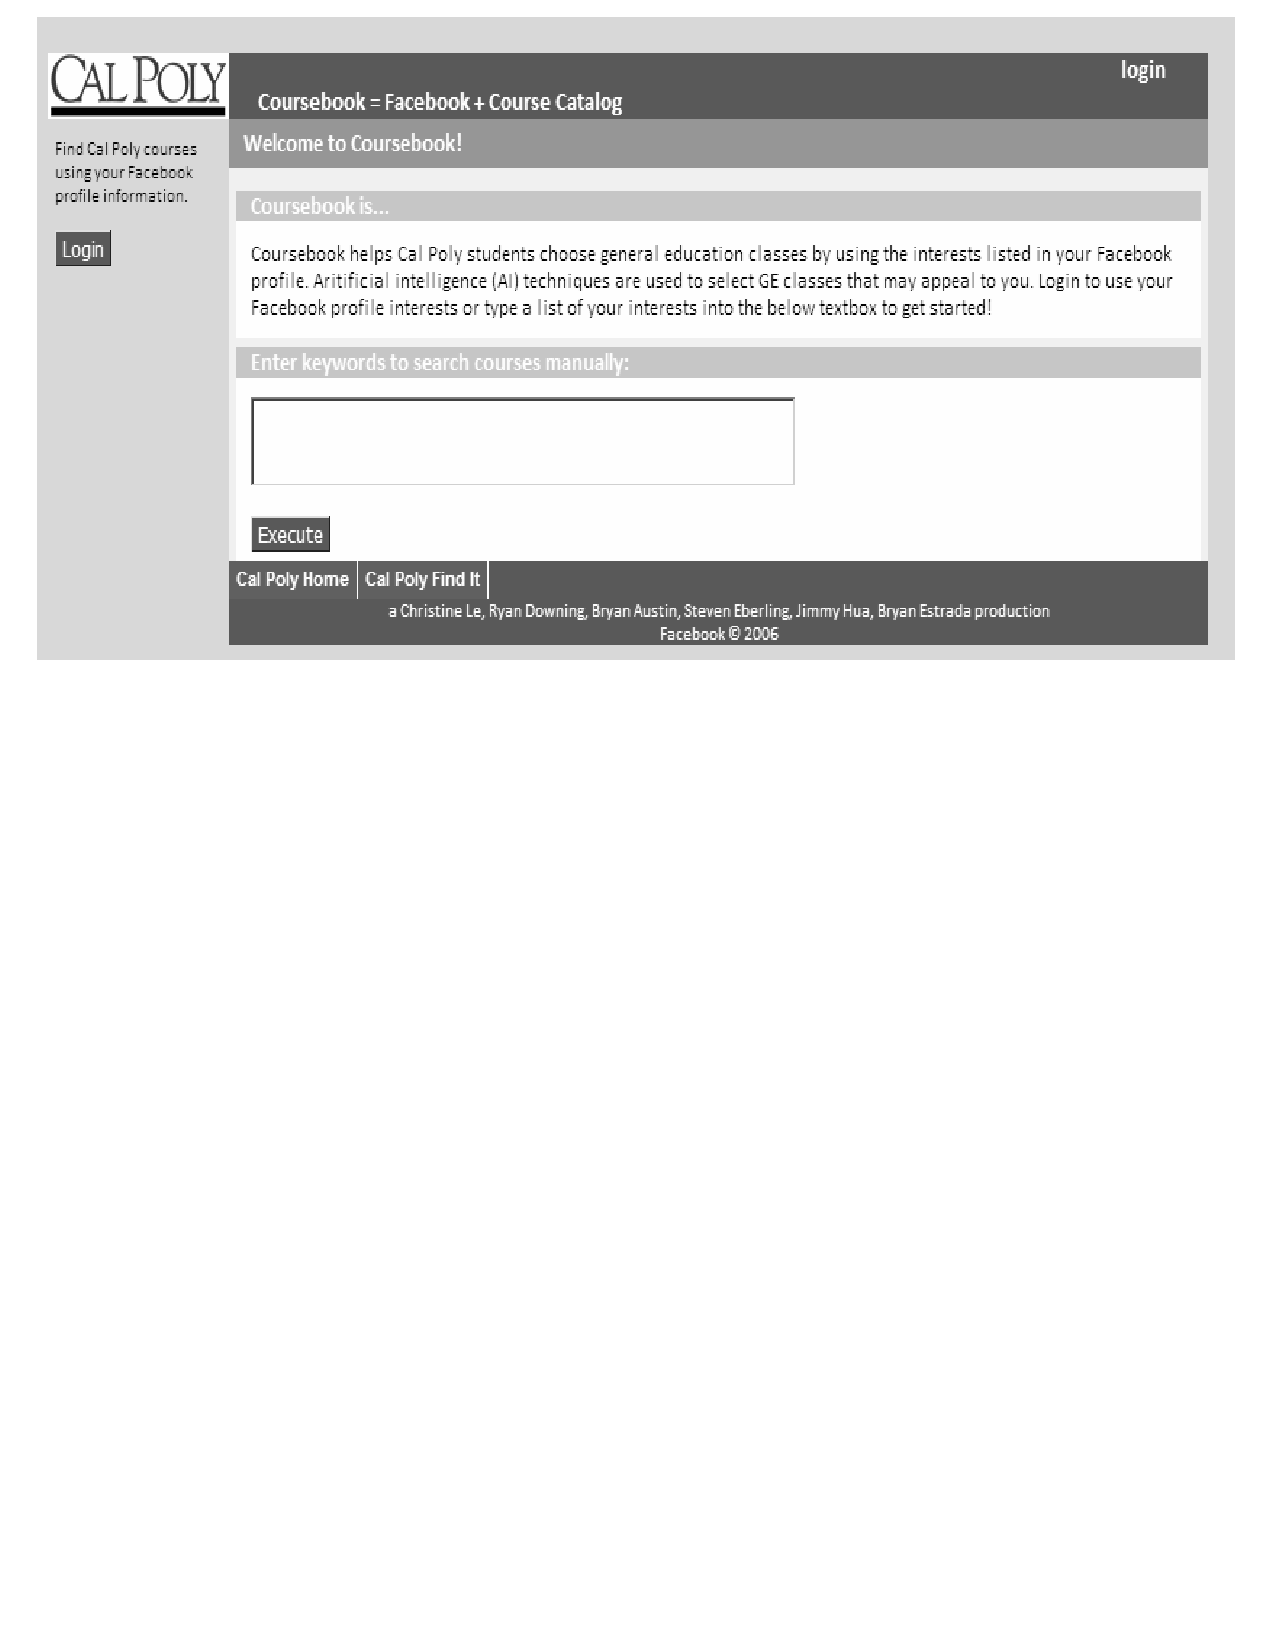
\includegraphics[scale=0.75]{images/screenshot}
  \caption{Coursebook Screenshot}
  \label{fig:screenshot}
  \end{center}
\end{figure}

\subsubsection*{Web User Interface}
By implementing Coursebook with a web-based user interface, we present users 
with an easily accessible service. Coursebook utilizes the latest technologies 
on the J2EE stack, including the Spring framework, JDBC, and WordNet APIs to 
produce a highly responsive system that is platform agnostic on both the server
side (Java) and client side (DHTML/Javascript).

\subsubsection*{Live Data}
Coursebook consists of multiple distributed components to provide users with 
information. The system relies on a MySQL database for real-time course catalog
information. The Facebook API provides developers access to its users' profile 
information. Coursebook offers multiple points of entry, including automatic 
Facebook connectivity and manual user input, in case the former system is 
inaccessible.

\subsubsection*{Relevant Courses}
Coursebook uses advanced artificial intelligence techniques to search and 
compute the most applicable courses for each individual user.

\section{Distributed Components}
\begin{figure}[t]
  \begin{center}
  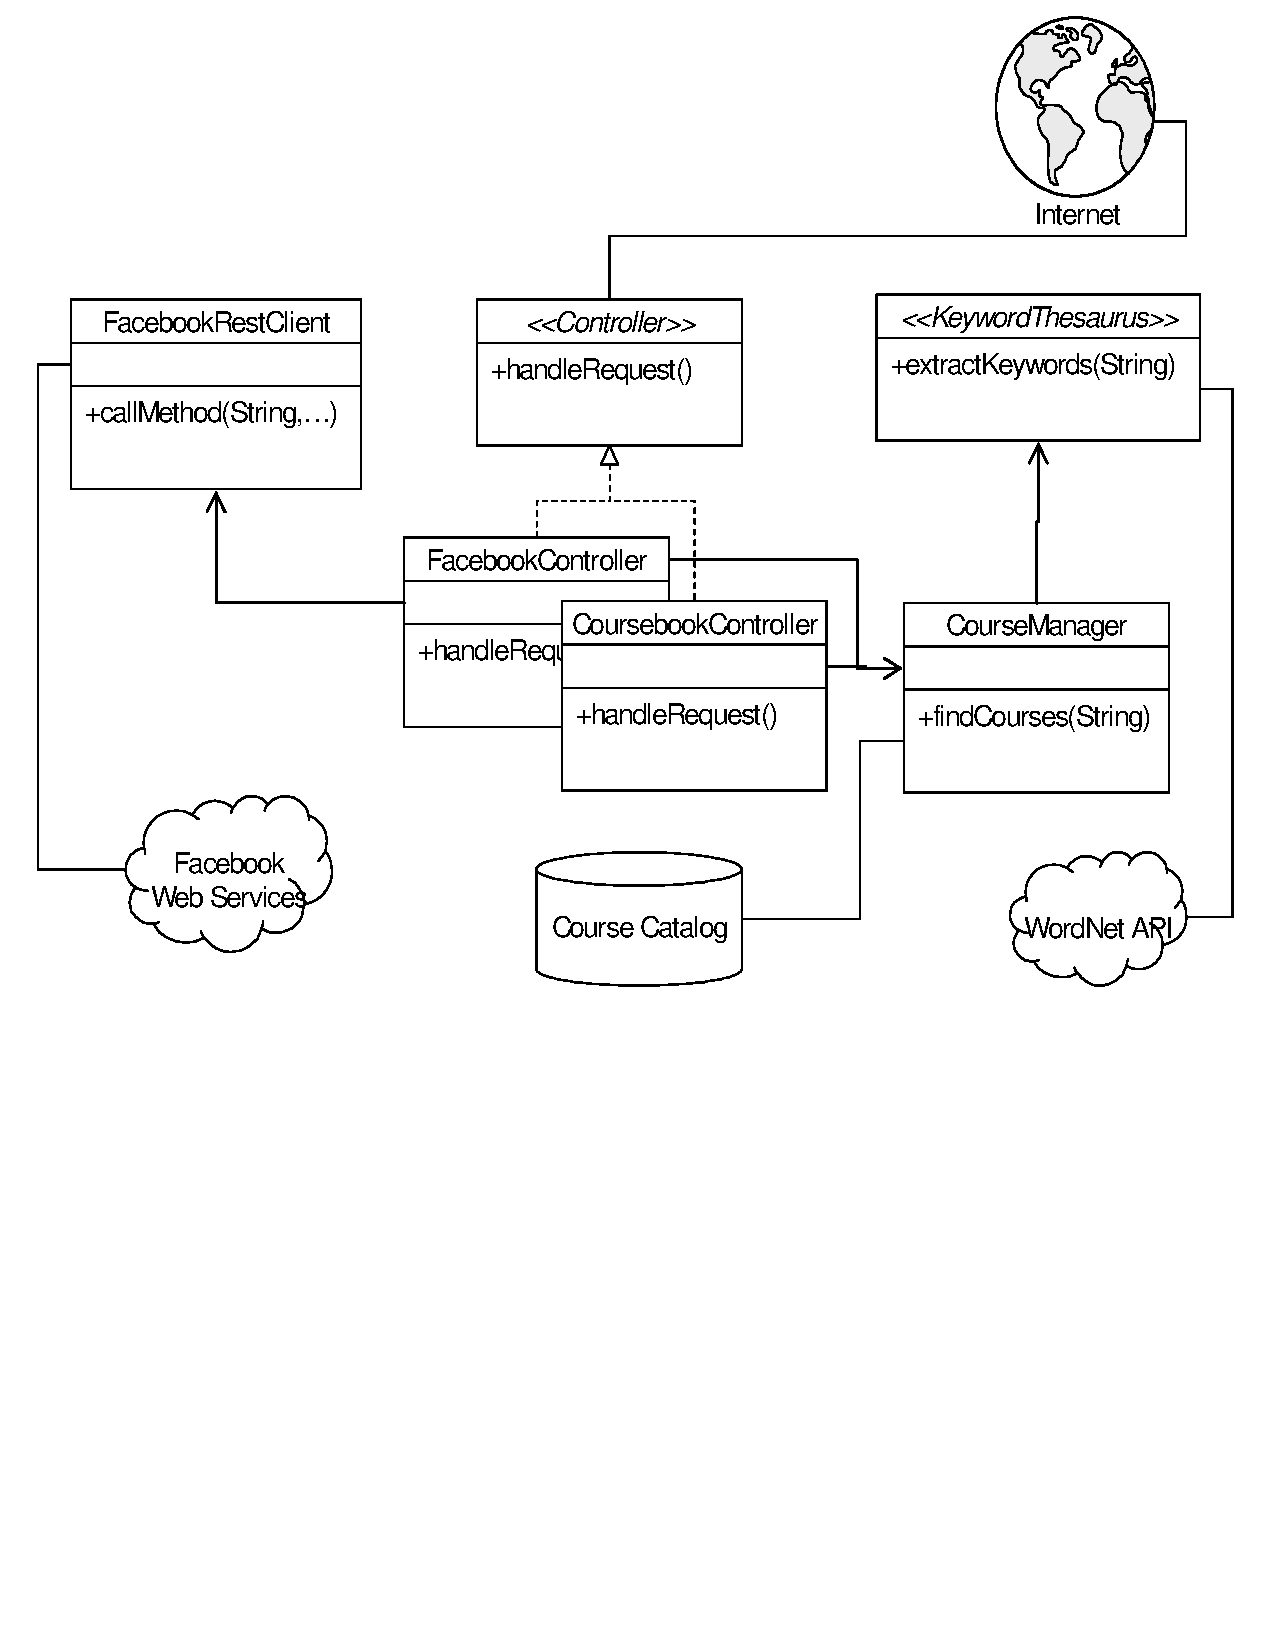
\includegraphics[width=\textwidth]{images/classes}
  \caption{Coursebook Abridged Class Diagram}
  \label{fig:classes}
  \end{center}
\end{figure}


